\documentclass[conference]{IEEEtran}
\IEEEoverridecommandlockouts

\usepackage{fancyhdr}
\pagestyle{fancy}
\fancyhf{}

\renewcommand{\thepage}{\Roman{page}} % Capital Roman numerals

\fancyhead[L]{\thepage}                 % Page number on left
\fancyhead[C]{A. SEN, S. VERMA, S. TULSYAN \& S. DHANUKA}

\usepackage{cite}
\usepackage{amsmath,amssymb,amsfonts}
\usepackage{algorithmic}
\usepackage{graphicx}
\usepackage{textcomp}
\usepackage{xcolor}
\usepackage{booktabs}
\usepackage{multirow}

\newcommand{\Var}{\mathrm{Var}}
\newcommand{\R}{\mathbb{R}}

\begin{document}

\title{Quantitative Analysis of Media Bias and Stock Price Dynamics: The 2020 Shock}

\author{\small
\begin{minipage}[t]{0.48\textwidth}
\centering
Anirban Sen \\
\textit{Dept of CS} \\
\textit{Ashoka University} \\
Sonipat, India \\
anirban.sen@ashoka.edu.in
\end{minipage}
\hfill
\begin{minipage}[t]{0.48\textwidth}
\centering
Shivansh Verma \\
\textit{Dept of CS} \\
\textit{Ashoka University} \\
Sonipat, India \\
shivansh.verma\_ug2023@ashoka.edu.in
\end{minipage}
\\[0.6em]
\begin{minipage}[t]{0.48\textwidth}
\centering
Soham Tulsyan \\
\textit{Dept of CS} \\
\textit{Ashoka University} \\
Sonipat, India \\
soham.tulsyan\_ug2023@ashoka.edu.in
\end{minipage}
\hfill
\begin{minipage}[t]{0.48\textwidth}
\centering
Sashwat Dhanuka \\
\textit{Dept of CS} \\
\textit{Ashoka University} \\
Sonipat, India \\
sashwat.dhanuka\_ug2023@ashoka.edu.in
\end{minipage}
}

\maketitle

\thispagestyle{empty}

\begin{abstract}
This paper studies how media reporting about large-cap firms changed around the 2020 recession and whether shifts in news stance predict firm-level stock outcomes. Using a large-scale NewsMTSC pipeline to compute daily stance scores from full-text news articles (2015--2025) for S\&P 500 firms, we combine NLP-derived stance with firm-day controls and market variables to test structural shifts, causal responses, and predictive linkages. Our identification strategy centers on a pre/post shock design around January 2020, complemented by difference-in-differences, interrupted time series, and time-series VAR exercises. We document the data pipeline, relevance filtering, stance aggregation, and robustness checks used throughout the analysis.
\end{abstract}

\section{Introduction}
The 2020 recession is a natural breakpoint for studying the interaction between media narratives and financial markets. COVID-era coverage expanded in volume and intensity, and a growing body of evidence documents a structural change in news-market dynamics during and after the shock. This project asks a simple, high-level question: did the tone of firm-specific media reporting shift after 2020, and if it did, did markets respond differently to that tone?

We approach the problem with a target-dependent stance framework rather than generic sentiment. NewsMTSC allows us to score whether an article is positive or negative toward a specific firm even when multiple firms are mentioned in the same text. That distinction is central to firm-level testing: a general sentiment score cannot distinguish positive coverage of one firm from negative coverage of another in the same article. Target-dependent stance makes it feasible to construct a daily, firm-level media stance signal and evaluate how it behaves across time and shocks.

The study is grounded in three observations from the project work so far. First, the 2020 shock is widely documented as a period in which media coverage and market behavior changed in a persistent way. Second, the data pipeline needs to be precise: naive keyword search introduces many false positives and inflates noise in the stance signal. Third, if stance is to be linked to returns in a credible way, the design must rule out coverage volume effects, pre-trend differences, and spurious correlations driven by macro shocks.

We therefore build a two-stage pipeline: (i) relevance classification that filters articles to those that actually report on the target firm, and (ii) NewsMTSC stance scoring with confidence thresholds. With this signal we pose three research questions on structural shifts in stance and returns and the post-shock stance-return linkage. Our empirical strategy combines pre/post regressions, interrupted time series, difference-in-differences, VAR and Granger causality, and event studies to triangulate the stance-return channel.

The remainder of the paper proceeds as follows. Section II defines research questions and hypotheses. Section III provides the data story and pipeline. Section IV lays out the methodology and identification strategy. Section V discusses validity threats and robustness. Section VI concludes with planned deliverables.

\section{Research Questions and Hypotheses}
We formalize three research questions (RQs) that map directly to the project pipeline.

\textbf{RQ1: Structural shift in media stance.} How did media reporting (stance) toward large-cap firms change pre versus post the 2020 recession? \\
\textbf{H1:} The 2020 shock induced a systematic shift in average daily stance scores after January 2020, conditional on firm fixed effects and controls.

\textbf{RQ2: Structural shift in returns.} Did the same shock change stock return behavior at the firm level? \\
\textbf{H2:} Mean firm-day returns shifted after 2020, even after controlling for market returns and volatility.

\textbf{RQ3: Post-shock sensitivity.} Did the stance-to-return relationship strengthen after 2020? \\
\textbf{H3:} The stance-to-return elasticity increased in the post-2020 period for S\&P 500 firms.

\section{Data and Signal Construction}
\subsection{Corpus and Coverage}
We begin with a large corpus of scraped full-text news articles (2015--2025). The core sample focuses on large-cap firms that are consistently observable across time, namely the S\&P 500. Articles are stored with publication, timestamp, URL, title, first paragraph, and full body text. We de-duplicate on titles and keep a separate record of filtered-out content to preserve traceability.

To avoid severe imbalance across firms and time, we use a stratified design: for each year we compute article counts per firm, take the minimum feasible count across firms, and sample to match that count. This preserves coverage across firms while avoiding a signal driven by a handful of highly covered companies.

\subsection{Sampling and Stratification (Facts and Figures)}
The starting panel contains 4,706,589 firm-article links across the top firms and years 2015--2025 (Table~\ref{tab:yearly_matrix}). This raw panel is highly skewed: some firms dominate the coverage while others have sparse years.

We therefore impose two sampling constraints. First, we filter to articles whose titles explicitly contain the company name or ticker and de-duplicate by normalized title per company (title-level deduplication). Second, we select firms that meet a minimum annual coverage threshold: a company is kept if it has at most three years with \(\leq 3000\) articles; companies failing this criterion are dropped (Table~\ref{tab:company_filter}). This yields a retained set of 22 companies and a stratified, filtered corpus of 483,514 firm-article links (Table~\ref{tab:filtered_matrix}).

\begin{table*}[htbp]
\caption{Yearly article totals in the starting panel (2015--2025)}
\label{tab:yearly_matrix}
\centering
\begin{tabular}{lrrrrrrrrrrr}
\toprule
Year & 2015 & 2016 & 2017 & 2018 & 2019 & 2020 & 2021 & 2022 & 2023 & 2024 & 2025 \\
\midrule
Total articles & 570,999 & 625,582 & 652,741 & 525,259 & 559,027 & 363,962 & 291,144 & 260,115 & 204,281 & 204,007 & 449,472 \\
\bottomrule
\end{tabular}
\end{table*}

\begin{table}[htbp]
\caption{Coverage filter for firm selection}
\label{tab:company_filter}
\centering
\begin{tabular}{lrr}
\toprule
Group & Firms & Rule \\
\midrule
Kept & 22 & At most three years with \(\leq 3000\) articles \\
Dropped & 8 & More than three years with \(\leq 3000\) articles \\
\bottomrule
\end{tabular}
\end{table}

\begin{table}[htbp]
\caption{Sample size after filtering and stratification}
\label{tab:filtered_matrix}
\centering
\begin{tabular}{lr}
\toprule
Stage & Total firm-article links \\
\midrule
Starting panel & 4,706,589 \\
Final stratified panel & 483,514 \\
\bottomrule
\end{tabular}
\end{table}

Figure~\ref{fig:article_count_distribution} shows the long-tail distribution of article counts per company, motivating stratification. Figure~\ref{fig:top20_articles} summarizes the top-coverage firms in the retained panel.

\begin{figure}[htbp]
\centerline{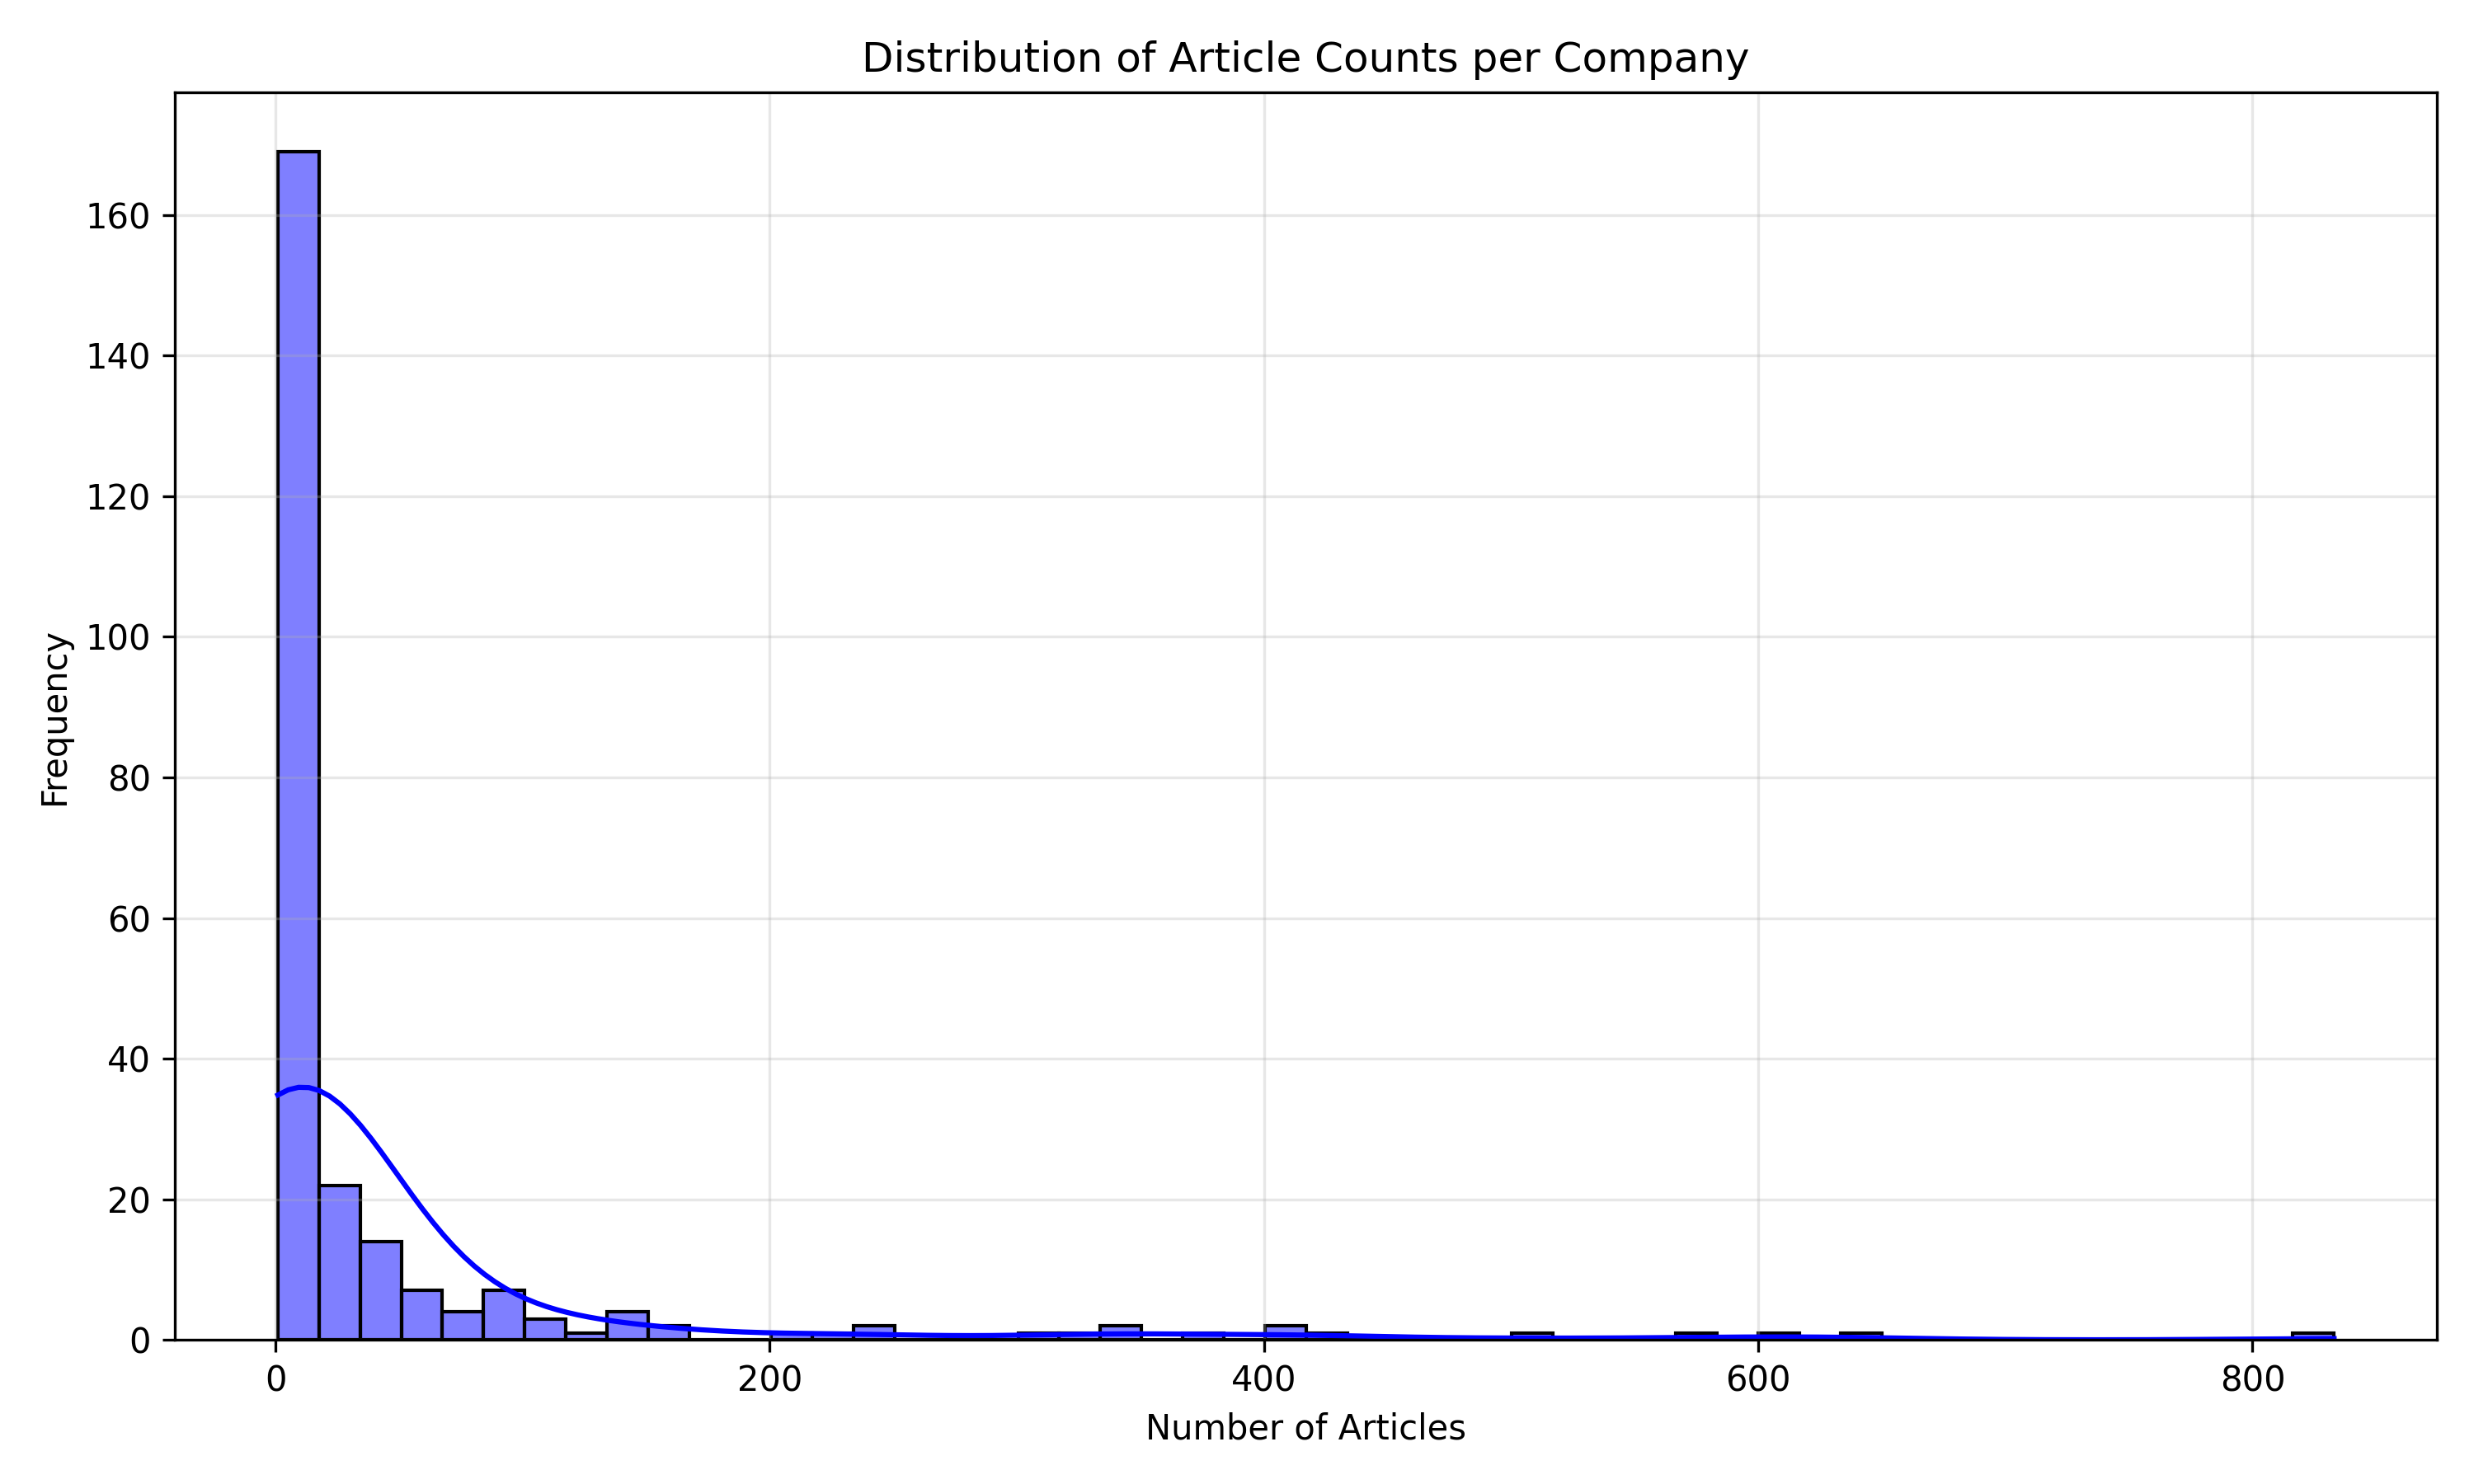
\includegraphics[width=\linewidth]{article_count_distribution.png}}
\caption{Distribution of article counts per company. The long tail motivates stratified sampling to avoid coverage-driven bias.}
\label{fig:article_count_distribution}
\end{figure}

\begin{figure}[htbp]
\centerline{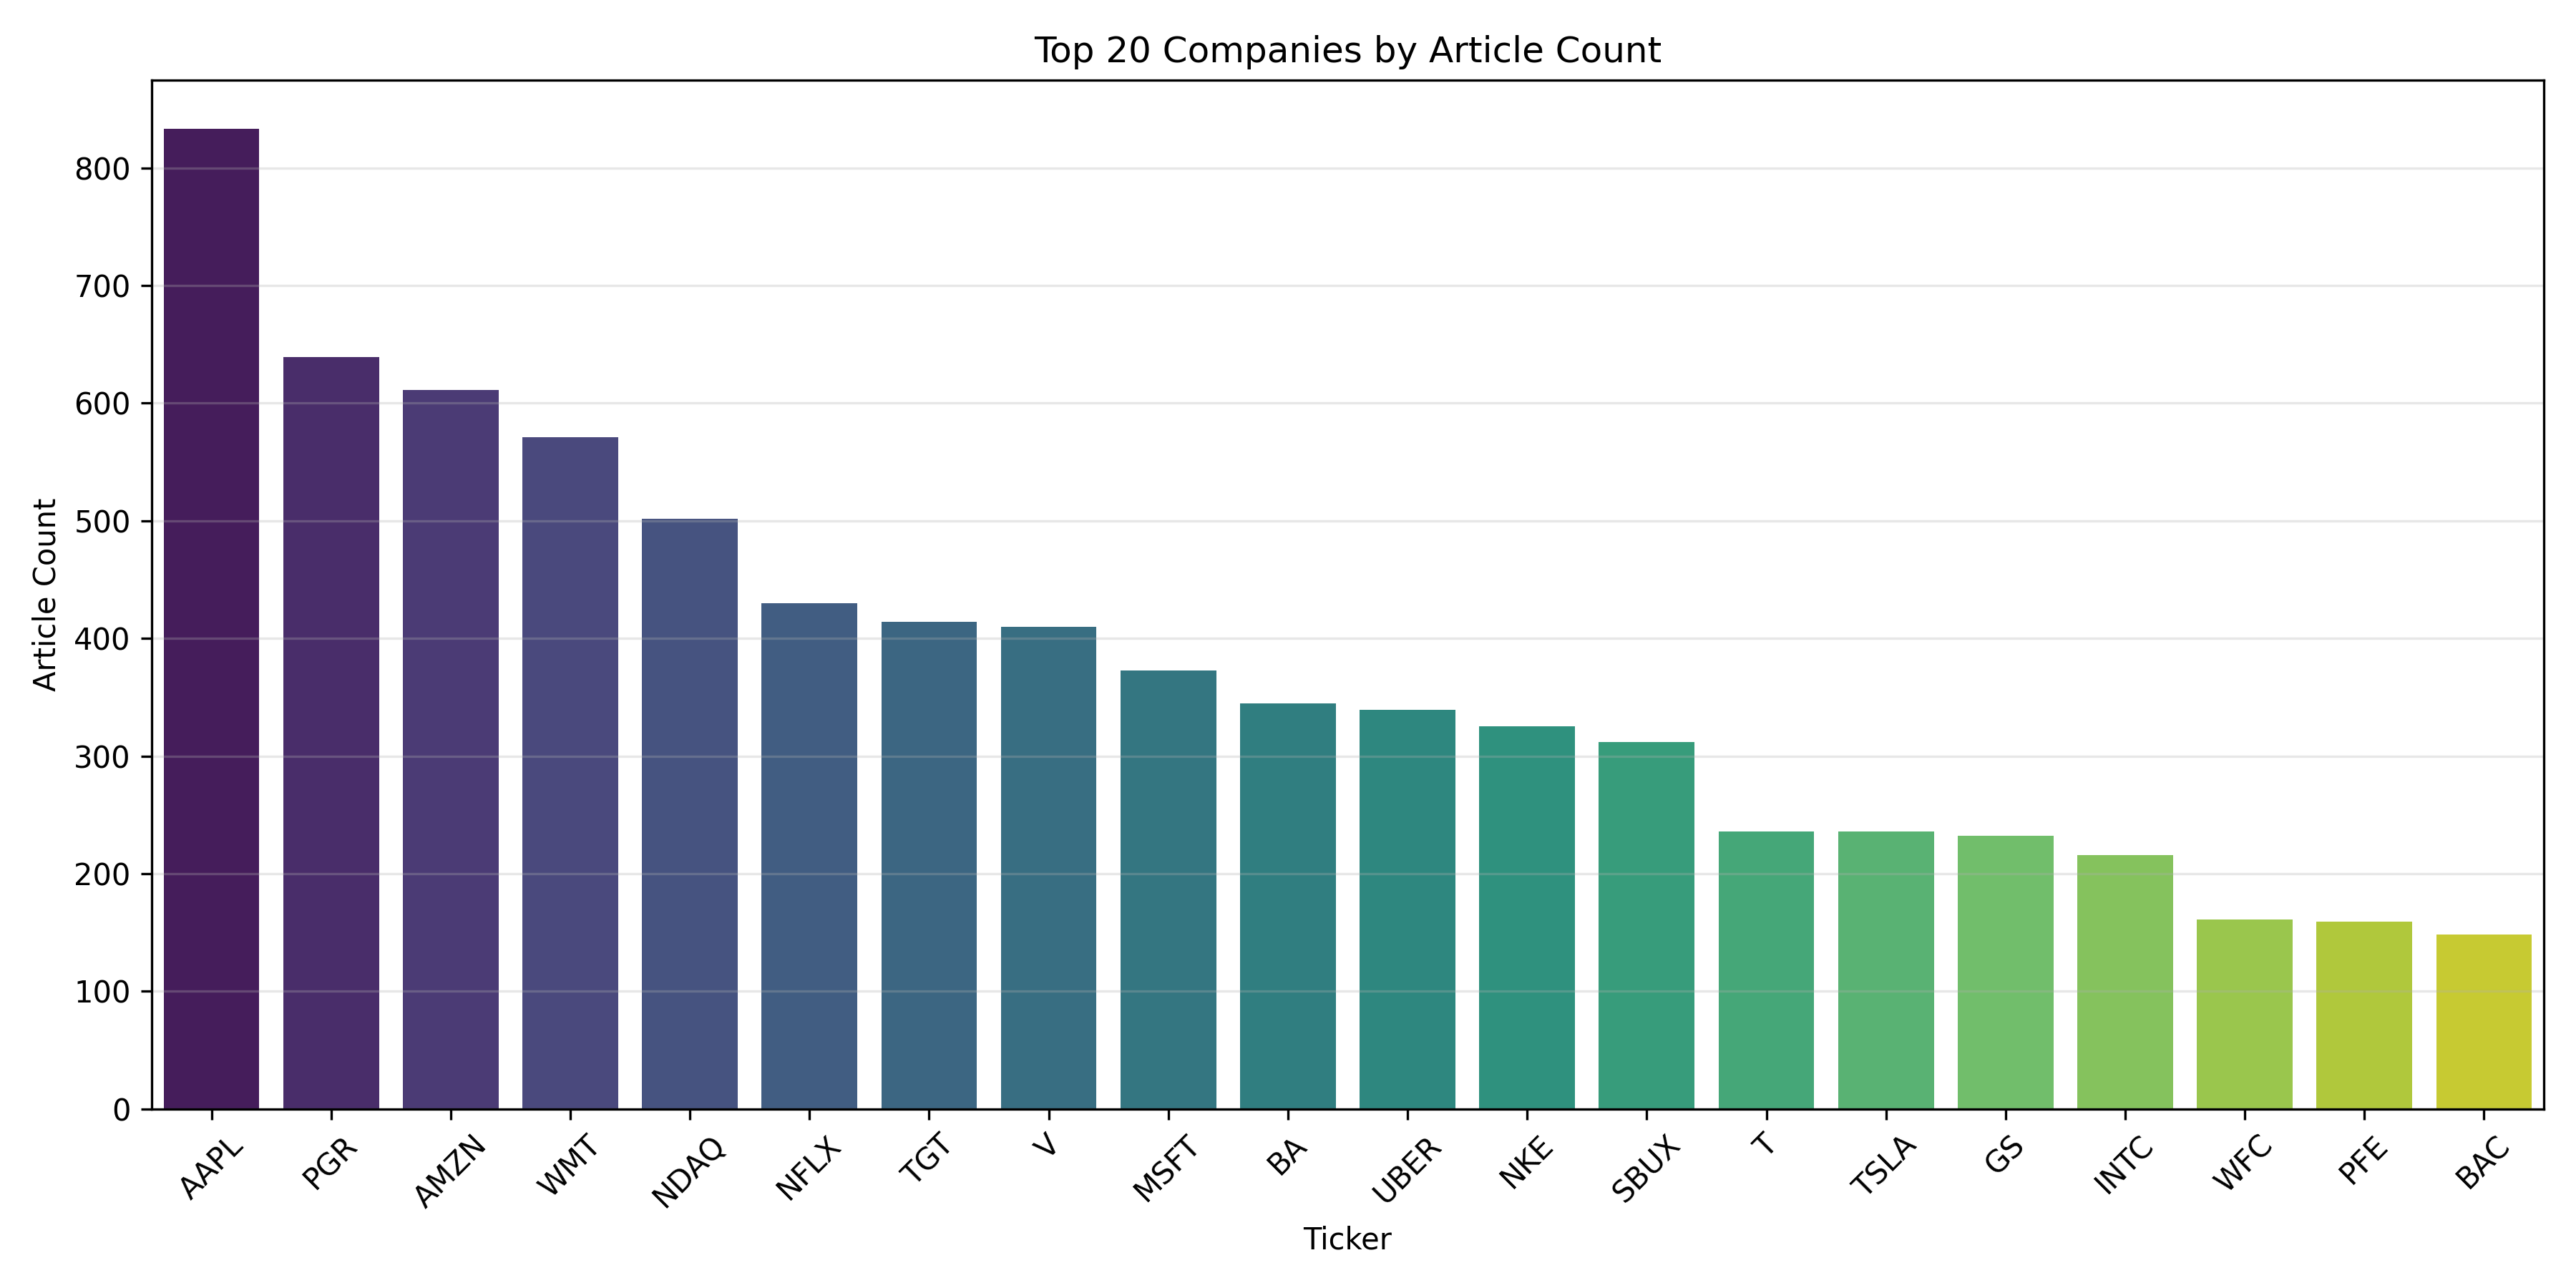
\includegraphics[width=\linewidth]{top_20_articles.png}}
\caption{Top 20 firms by article count in the retained sample.}
\label{fig:top20_articles}
\end{figure}

\subsection{Relevance Filtering and Annotation}
Keyword matching is not enough for firm targeting (e.g., ``Apple'' is not always the company). We therefore apply a two-stage relevance pipeline: (i) title-based pre-filtering that retains only articles with the company name in the title (company names, not tickers), and (ii) a supervised relevance classifier trained on manual annotations. The held-out test set for manual annotation is kept completely separate from training.

Our base classifier is DeBERTa-v3 fine-tuned for binary classification using article titles. The first model, trained on 750 labeled articles, achieved high recall but insufficient precision. We then expanded the training data via semi-supervised mining: running the model on a large unlabeled pool and adding only high-confidence predictions ($p_{rel} \ge 0.92$ for relevant, $p_{rel} \le 0.05$ for irrelevant). This expanded set increases precision and reduces false positives. An ensemble of model variants further improves precision, and the operating threshold is selected via a sweep to meet a target of precision $\ge 0.90$.

\subsection{Stance Scoring}
Stance is computed using the NewsMTSC model for target-dependent stance. For each qualifying article we obtain probabilities for positive, negative, and neutral stance. The baseline specification retains only high-confidence outputs (prob >= 0.9), and we report sensitivity to lower thresholds (0.6 and 0.0). Daily firm-level stance is the average across articles on that day:
\begin{equation}
\text{stance}_{i,t} = \frac{1}{N_{i,t}} \sum_{a \in A_{i,t}} (p^{+}_{a} - p^{-}_{a})
\end{equation}
where $A_{i,t}$ is the set of high-confidence articles for firm $i$ on day $t$ and $N_{i,t}$ is the count. We also construct article volume and coverage mix covariates to separate tone shifts from coverage shifts.

\subsection{Market Alignment and Controls}
The stance series is aligned to firm-day market outcomes: daily returns, S\&P 500 index returns, and VIX. We also log-normalize article volume in regressions. This alignment yields the panel used across the RQ1--RQ3 specifications.

\section{Methodology}
This section groups the empirical strategy into three layers: (i) structural shifts around the 2020 shock, (ii) stance-return linkage, and (iii) time-series dynamics and event studies.

\subsection{RQ1: Stance Shift Around the 2020 Shock}
We test for a structural shift in stance using a pre/post specification with firm fixed effects:
\begin{equation}
\text{stance}_{i,t} = \alpha_i + \beta \cdot Post_t + \gamma' X_{i,t} + \varepsilon_{i,t}
\end{equation}
where $Post_t$ equals 1 after January 2020 (post period: 2020--2025; pre: 2015--2019) and $X_{i,t}$ includes article volume and VIX. If pre-period means are not comparable, we implement Synthetic Control DiD (SCDiD) or use an interrupted time-series specification with level and trend shifts.

\subsection{RQ2: Returns Shift Around the 2020 Shock}
The returns analogue mirrors the stance regression, with returns as the outcome and market controls added:
\begin{equation}
\text{return}_{i,t} = \alpha_i + \beta\,\text{Post}_t + \gamma' X_{i,t} + \varepsilon_{i,t}
\end{equation}
where $X_{i,t}$ includes index returns and VIX to absorb market-wide shocks.

\subsection{RQ3: Stance-Return Linkage}
We test the direct stance-return relationship using next-day returns:
\begin{equation}
\text{return}_{i,t+1} = \alpha_i + \beta\,\text{stance}_{i,t} + \gamma' X_{i,t} + \varepsilon_{i,t}
\end{equation}
To test whether the stance-to-return sensitivity changes post-2020, we use a triple interaction:
\begin{equation}
\begin{aligned}
\text{return}_{i,t} &= \alpha_i + \beta\,\text{Post}_t + \gamma\,\text{stance}_{i,t} \\
&\quad + \delta(\text{Post}_t \times \text{stance}_{i,t}) + \theta X_{i,t} + \varepsilon_{i,t}
\end{aligned}
\end{equation}
where the interaction $\text{Post}_t \times \text{stance}_{i,t}$ captures post-shock amplification of the stance-return channel.

\subsection{Time-Series Dynamics and Event Studies}
We estimate VARs on (stance, returns) to capture bidirectional dynamics and compute impulse response functions. Granger causality tests evaluate whether past stance improves return forecasts beyond past returns, and whether the reverse also holds. We also test for autocorrelation in stance using ARIMA models, which motivates lagged stance controls.

As a non-parametric check, we run event studies around large stance jumps (e.g., >2 SD from a rolling mean) and compute abnormal returns in short windows around those events.

\subsection{Robustness and Sensitivity}
We perform numerous robustness checks: alternative stance aggregation (median, winsorized means), different confidence thresholds, exclusion of low-coverage firm-days, placebo pre/post cutoffs, and treatments that control for article topical composition. We also test sensitivity to training-test splits for the relevance classifier and manual annotation thresholds.

\section{Regression Analysis}
This section develops the panel regression framework used to test the first two
research questions: whether firm-level media stance (RQ1) and firm-level stock
returns (RQ2) exhibit a structural shift around the 2020 recession. Both
questions share a common pre/post design built on a fixed-effects panel
estimator, which is the natural workhorse for repeated observations of the same
firms over time. We describe variable construction, the estimating equations,
the estimator and its inference, and the diagnostic battery used to certify that
the estimates satisfy the classical linear model (CLM) assumptions.

\subsection{Variable Construction}
The unit of analysis is the firm--day pair $(i,t)$. For each scored article $a$
of firm $i$ published on date $t$, the NewsMTSC model returns a probability
triple $(p_a^{+}, p_a^{-}, p_a^{0})$ over the positive, negative, and neutral
stance classes toward the target firm. We collapse this triple into a signed
article-level stance,
\begin{equation}
s_a = p_a^{+} - p_a^{-},
\end{equation}
which lies in $[-1,1]$ and is large in magnitude only when the model is
confident and one-sided. The firm--day media stance, our RQ1 outcome, is the
simple mean of article stances on that day,
\begin{equation}
\text{bias}_{it} = \frac{1}{|\mathcal{A}_{it}|}\sum_{a\in\mathcal{A}_{it}} s_a,
\end{equation}
where $\mathcal{A}_{it}$ is the set of qualifying articles for firm $i$ on day
$t$. Optionally only high-confidence articles
$\max\{p_a^{+},p_a^{-},p_a^{0}\}\ge\tau$ are retained; the headline RQ1
specification sets $\tau=0$ to maximize coverage, and lower-coverage thresholds
($\tau=0.6,0.9$) are used as sensitivity checks.

The RQ2 outcome is the firm--day simple return computed from adjusted close
prices,
\begin{equation}
\text{return}_{it} = \frac{P_{it}-P_{i,t-1}}{P_{i,t-1}}.
\end{equation}
The treatment variable common to both questions is the post-shock indicator
\begin{equation}
\text{Post}_t = \mathbf{1}[\,t \ge \text{2020-01-01}\,],
\end{equation}
which partitions the panel into a pre-period (2015--2019) and a post-period
(2020--2025). The remaining regressors are controls chosen to absorb confounders
that would otherwise contaminate the post coefficient. For RQ1 we include
firm--day article volume $\text{vol}_{it}=|\mathcal{A}_{it}|$, because the mean
of a noisy stance signal mechanically tightens as more articles are averaged, so
volume must be held fixed to separate a genuine tone shift from a coverage
shift. For RQ2 we include the contemporaneous S\&P 500 index return
$\text{sp500\_return}_t$, which absorbs the market-wide bull-run and broad index
drift, and the volatility index $\text{vix}_t$, which absorbs common
volatility-regime shifts. Without these two controls the post indicator would
simply re-estimate the average market path before and after 2020 rather than the
firm-specific component of interest.

\subsection{Estimating Equations}
RQ1 is estimated with a two-way fixed-effects specification,
\begin{equation}
\text{bias}_{it} = \alpha_i + \delta_t + \beta\,\text{Post}_t
+ \gamma\,\text{vol}_{it} + \varepsilon_{it},
\label{eq:rq1twfe}
\end{equation}
where $\alpha_i$ are firm fixed effects and $\delta_t$ are daily time fixed
effects. The firm effects absorb every time-invariant firm characteristic (an
outlet's structural tendency to cover a given firm favorably), while the day
effects absorb every firm-invariant daily shock (market-wide sentiment swings or
macro news). With both sets of dummies present, $\beta$ identifies only the
idiosyncratic within-firm shift in stance after 2020 that is orthogonal to
common daily movements. Because $\text{Post}_t$ is itself a function of the
calendar, $\beta$ is identified through the interaction of the step with the
firm dimension once daily effects are partialled out.

RQ2 mirrors this design with an entity (firm) fixed-effects specification and
market controls,
\begin{equation}
\text{return}_{it} = \alpha_i + \beta\,\text{Post}_t
+ \gamma_1\,\text{sp500\_return}_t + \gamma_2\,\text{vix}_t + \varepsilon_{it}.
\label{eq:rq2fe}
\end{equation}
Here the firm effects remove permanent cross-firm differences in mean return,
and the two market controls strip out the systematic component of returns so
that $\beta$ measures the firm-idiosyncratic post-2020 mean shift.

\subsection{Estimator and Inference}
Both models are estimated by the within (Mundlak) transformation: each variable
is demeaned by its firm and, for RQ1, time means, and ordinary least squares is
applied to the transformed data,
\begin{equation}
\hat{\theta} = (\tilde{X}^{\top}\tilde{X})^{-1}\tilde{X}^{\top}\tilde{y},
\end{equation}
where tildes denote within-transformed quantities and $\theta=(\beta,\gamma)^\top$.
This is algebraically identical to dummy-variable OLS but avoids storing
thousands of fixed-effect columns, which is essential given $26$ firms and over
$4{,}000$ daily periods. Standard errors use the heteroscedasticity-robust HC1
estimator,
\begin{equation}
\widehat{\Var}(\hat{\theta}) = \frac{n}{n-K}(\tilde{X}^{\top}\tilde{X})^{-1}
\Bigl(\textstyle\sum_{j=1}^{n}\hat{u}_j^{2}\,\tilde{x}_j\tilde{x}_j^{\top}\Bigr)
(\tilde{X}^{\top}\tilde{X})^{-1},
\end{equation}
and two-sided $p$-values are obtained from the normal approximation
$p_k = 2\,\Phi(-|t_k|)$ with $t_k=\hat{\theta}_k/\widehat{\mathrm{SE}}(\hat{\theta}_k)$.
Because the panel is observed daily and firms are exposed to common trading-day
shocks, we additionally report day-clustered standard errors for RQ1, which are
robust to arbitrary cross-firm correlation within the same trading day and are
our preferred uncertainty estimate for the static model.

\subsection{RQ1 Results}
Table~\ref{tab:rq1} reports the two-way fixed-effects estimates. The post
coefficient is positive ($0.0141$) but statistically insignificant
($p=0.30$), while article volume is strongly negative and highly significant,
confirming that heavier coverage is associated with more neutral average tone
within a firm--day. Day-clustered inference (SE $=0.0134$) is almost identical to
the HC1 result, indicating that within-day cross-firm dependence does not
materially affect the conclusion.

\begin{table}[!t]
\caption{RQ1: Two-Way Fixed-Effects Estimates of Media Stance ($\alpha_i+\delta_t$)}
\label{tab:rq1}
\centering
\small
\begin{tabular}{lrrr}
\toprule
Variable & Coef. & SE (HC1) & $p$-value \\
\midrule
Post            & $0.014130$  & $0.013623$ & $0.2996$ \\
Article Volume  & $-0.000970$ & $0.000076$ & $<0.0001$ \\
\midrule
\multicolumn{4}{l}{Firm--day obs. $n=63{,}200$; Firms $=26$; Days $=4{,}018$} \\
\multicolumn{4}{l}{Raw articles after filters $=690{,}586$; Within $R^2=0.0017$} \\
\bottomrule
\end{tabular}
\end{table}

The weakness of the static post coefficient is itself informative rather than a
failure of the design. An $F$-test of the $4{,}017$ daily fixed effects against a
firm-only model is jointly significant ($F=1.135$ versus a $5\%$ critical value
of $1.038$, $p=1.1\times10^{-8}$), so daily shocks clearly drive much of the
temporal variation in stance. Because those daily dummies absorb most of the
common-time movement, the coarse stepwise $\text{Post}_t$ indicator is left with
little residual variation to explain, which both attenuates $\beta$ and keeps the
within $R^2$ small; the within $R^2$ measures only the share of demeaned variance
explained, and firm--day stance is dominated by idiosyncratic article noise.

To recover the timing that the single step compresses, we estimate a monthly
event study with firm effects, article volume, and month-relative dummies around
January 2020 (reference month $m=-1$, December 2019). Table~\ref{tab:rq1es}
reports the informative horizons. Pre-shock coefficients are small and
insignificant, consistent with the parallel-trends premise, whereas the
post-shock coefficients build gradually and become significant from roughly three
months onward, peaking at $m=+12$ ($0.064$, $p<0.001$) and remaining elevated at
$m=+24$. The 2020 effect is therefore a slow, persistent uplift rather than a
single discrete jump, which explains why the static post term is muted once daily
effects are absorbed.

\begin{table}[!t]
\caption{RQ1: Selected Monthly Event-Study Coefficients (Firm FE)}
\label{tab:rq1es}
\centering
\small
\begin{tabular}{lrrrl}
\toprule
Month & Coef. & SE (HC1) & $p$-value & Phase \\
\midrule
$m=-12$ & $0.021692$ & $0.018045$ & $0.2293$ & pre-trend \\
$m=-6$  & $0.031757$ & $0.017201$ & $0.0649$ & pre-trend \\
$m=0$   & $0.031032$ & $0.018354$ & $0.0909$ & event \\
$m=+3$  & $0.042152$ & $0.019168$ & $0.0279$ & early post \\
$m=+6$  & $0.032197$ & $0.018248$ & $0.0777$ & mid post \\
$m=+12$ & $0.064054$ & $0.018797$ & $0.0007$ & persistent \\
$m=+24$ & $0.050394$ & $0.018705$ & $0.0071$ & long-run \\
\bottomrule
\end{tabular}
\end{table}

\subsection{RQ1 Diagnostics (BLUE/CLM Checks)}
Table~\ref{tab:rq1mlr} summarizes the diagnostic battery used to certify the
estimator. The residual mean is numerically zero ($-9.0\times10^{-19}$),
confirming orthogonality, and the design is numerically well conditioned
(condition number $157.5$). Multicollinearity is negligible: both variance
inflation factors are $\approx 1.0$ and the maximum pairwise correlation is
$0.019$. Two assumptions are violated in the expected ways for financial panel
data: the Breusch--Pagan test rejects homoscedasticity (LM $=190.3$) and the
Jarque--Bera test rejects normality (JB $=4541$, kurtosis $4.25$, indicating fat
tails). Neither threatens the estimates: HC1 and day-clustered standard errors
already correct for heteroscedasticity, and with $n=63{,}200$ the central limit
theorem justifies the normal-approximation inference despite non-normal
residuals. The Durbin--Watson statistic ($1.67$) indicates mild serial
correlation that is partly absorbed by the time effects. The estimator is
therefore best linear unbiased under the Gauss--Markov conditions, with robust
inference applied where the ideal conditions fail.

\begin{table}[!t]
\caption{RQ1: Summary Diagnostics}
\label{tab:rq1mlr}
\centering
\footnotesize
\setlength{\tabcolsep}{3.5pt}
\begin{tabular}{lrl}
\toprule
Test & Statistic & Implication \\
\midrule
Residual mean        & $-9.0\times10^{-19}$ & Orthogonality OK \\
Condition number     & $157.46$ & Stable \\
Breusch--Pagan (LM)  & $190.25$ & Heteroscedastic (HC1 used) \\
Jarque--Bera         & $4541.18$ & Fat tails ($n$ large) \\
VIF (both regressors)& $\approx 1.00$ & No collinearity \\
Durbin--Watson       & $1.673$ & Mild autocorrelation \\
\bottomrule
\end{tabular}
\end{table}

\subsection{RQ2 Results}
The returns panel contains $62{,}667$ firm--day observations across $26$ firms
(2015-12-01 to 2025-11-24), with tightly clustered pre-period means (range
$0.0019$, SD $0.0004$). Table~\ref{tab:rq2} reports the entity fixed-effects
estimates. Conditional on the index return and VIX, the post-period shift in
daily firm returns is negative and marginally significant
($-0.000344$, $p=0.045$), corresponding to about $-0.034\%$ per day. The market
return loads strongly and significantly (a coefficient near unity, as expected
for large-cap constituents), confirming that the control is doing its job, while
VIX is insignificant once the index return is included. The contrast between
RQ1 and RQ2 is the substantive payoff: media stance shows a slow post-2020
uplift while raw returns show only a faint downward mean shift, motivating the
dynamic analysis in the next section, where the question becomes not whether
each series shifts in level but whether the lead--lag relationship between them
changes.

\begin{table}[!t]
\caption{RQ2: Entity Fixed-Effects Estimates of Daily Returns (HC1 Robust SE)}
\label{tab:rq2}
\centering
\small
\begin{tabular}{lrrr}
\toprule
Variable & Coef. & SE (HC1) & $p$-value \\
\midrule
Post           & $-0.000344$ & $0.000172$ & $0.0451$ \\
S\&P 500 Return& $1.127576$  & $0.010982$ & $<0.0001$ \\
VIX            & $-0.000001$ & $0.000020$ & $0.9654$ \\
\bottomrule
\end{tabular}
\end{table}

\subsection{Why This Design Fits the Study, and Its Limits}
The two-way fixed-effects panel is the appropriate estimator here because the
data are repeated firm--day observations in which the principal confounders are
either firm-permanent (outlet--firm coverage tendencies) or day-common
(market-wide news), exactly the two margins that firm and time dummies absorb by
construction. The pre/post step matches the research design, which targets a
single documented macro break (the 2020 recession), and the event-study
extension guards against the well-known limitation of a static
difference-in-means by exposing the timing and testing for pre-trends. Robust and
clustered standard errors keep inference valid under the heteroscedasticity and
within-day dependence that the diagnostics confirm.

Three limitations should temper the interpretation. First, identification rests
on a conditional within-firm parallel-trends assumption; the flat pre-shock
event-study coefficients are supportive but not a proof, and any firm-specific
trend coinciding with 2020 would bias $\beta$. Second, the stance signal inherits
the measurement error of the upstream NewsMTSC and relevance-classifier stages,
which adds classical noise that depresses the within $R^2$ and can attenuate
coefficients toward zero. Third, a binary post indicator cannot distinguish the
2020 shock from other contemporaneous regime changes, and the low explanatory
power of the static model means it is better read as evidence about the
\emph{shape} of the adjustment than as a precise effect size. These limitations
directly motivate the time-series approach that follows.

\section{Vector Autoregression and Granger Causality Analysis}
The regressions in the previous section ask whether the level of each series
shifts after 2020. They are silent on the dynamic relationship between media
stance and returns: whether past stance helps predict future returns, whether
returns feed back into coverage, and whether that lead--lag structure itself
changed after the shock. We answer these questions with a vector autoregression
(VAR) and Granger-causality framework, supported by an eight-stage data
pipeline that constructs a clean, stationarity-validated weekly panel before any
dynamic model is fit. We move to a weekly frequency for this analysis because
daily firm-level stance is sparse and noisy for several firms, whereas weekly
aggregation yields near-complete coverage (median $99.8\%$ of weeks) while
retaining enough observations ($\approx 522$ weeks per firm) for lag-rich models.

\subsection{The VAR Model}
For a firm with endogenous vector $\mathbf{y}_t=(\Delta\text{bias}_t,\,r_t)^{\top}$,
where $\Delta\text{bias}_t$ is the first difference of the weekly bias index and
$r_t$ is the weekly log return, a reduced-form VAR of order $p$ is
\begin{equation}
\mathbf{y}_t = \mathbf{c} + \sum_{\ell=1}^{p}\mathbf{A}_\ell\,\mathbf{y}_{t-\ell}
+ \mathbf{u}_t,
\label{eq:var}
\end{equation}
with coefficient matrices $\mathbf{A}_\ell\in\R^{2\times2}$ and innovations
$\mathbf{u}_t$ having covariance $\Sigma$. The off-diagonal entries of the
$\mathbf{A}_\ell$ carry the cross-dynamics: a nonzero $(1,2)$ entry means past
returns move current stance, and a nonzero $(2,1)$ entry means past stance moves
current returns. The VAR is the minimal model that treats both variables as
endogenous and lets the data, rather than an a priori causal ordering, reveal the
direction of predictability, which is precisely what a media--market feedback
question requires.

\subsection{Stage 1--4: Building the Weekly Panel}
The pipeline begins with a \emph{data inventory} (Stage 1) that audits, for every
candidate firm, article counts, coverage, and the share of zero-article days, and
flags sparse firms ($<30\%$ trading-day coverage) for exclusion. This audit
motivates the move to a weekly frequency and the retention of sixteen
well-covered firms. Stage 2 constructs the \emph{weekly bias index} by
aggregating signed article stances into ISO weeks and verifies distributional
quality (mean, skew, kurtosis, and the incidence of single-article weeks). Stage
3 performs \emph{gap analysis and imputation}: weekly gaps are classified by
length, with short Type-A gaps (1--2 weeks) forward-filled and medium Type-B gaps
(3--8 weeks) linearly interpolated, while long Type-C gaps are left missing; only
$58$ observations require imputation and all sixteen firms clear a $\ge 60\%$
coverage threshold with no gap exceeding eight weeks. Crucially, both an imputed
and an observed-only series are retained so that every downstream test can be
re-run to confirm results are not artifacts of imputation. Figure~\ref{fig:gap}
illustrates the coverage map for the sparsest retained firm.

\begin{figure}[!t]
\centerline{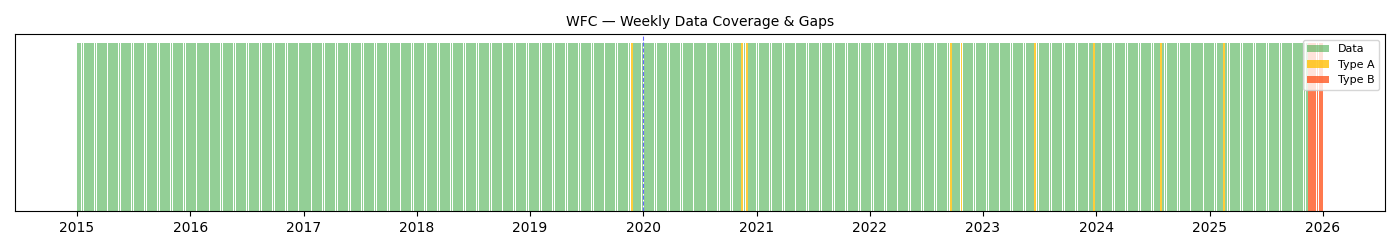
\includegraphics[width=\columnwidth]{fig_gap_WFC.png}}
\caption{Weekly data-coverage and gap map for Wells Fargo (WFC), the
lowest-coverage retained firm. Short and medium gaps are imputed; the series
still clears the $\ge 60\%$ coverage threshold.}
\label{fig:gap}
\end{figure}

Stage 4 constructs the \emph{returns series} as weekly log returns from
Monday-anchored ISO weeks and aligns them to the bias index. Log returns are used
because they are additive across time and approximately symmetric, which suits a
linear dynamic model. Quality checks flag extreme weekly moves
($>\pm15\%$, concentrated in the March 2020 crash window) for later
winsorization, and every firm clears the minimum of $100$ aligned weeks, yielding
a merged panel of $8{,}090$ firm--week rows.

\subsection{Stage 5: Stationarity and Cointegration}
A VAR in levels is only valid if the series are stationary or jointly
cointegrated; otherwise the regression is spurious. Each series is classified by
combining the Augmented Dickey--Fuller (ADF) test, whose null is a unit root, with
the KPSS test, whose null is stationarity. A series is called $I(0)$ when ADF
rejects ($p<0.05$) and KPSS does not, $I(1)$ in the opposite case, and
``conflicting'' (a likely structural break) when both reject. As expected for
financial data, weekly log returns are $I(0)$ for essentially every firm, while
the bias index is predominantly $I(1)$ or break-driven in levels but $I(0)$ in
first differences. This mixed integration order is the reason the VAR is
specified on $(\Delta\text{bias}_t,\,r_t)$ rather than on the levels: differencing
the bias index renders it stationary and avoids a spurious levels regression
against $I(0)$ returns. A Johansen trace test detects a cointegrating relation
only for Wells Fargo (trace $=340.2$ against a $95\%$ critical value of $15.5$),
which would otherwise call for a VECM; for the common $(\,I(1),I(0)\,)$ case
cointegration is impossible, confirming the differenced specification.
Figure~\ref{fig:stat} shows the level-versus-difference diagnostic for a
representative firm.

\begin{figure}[!t]
\centerline{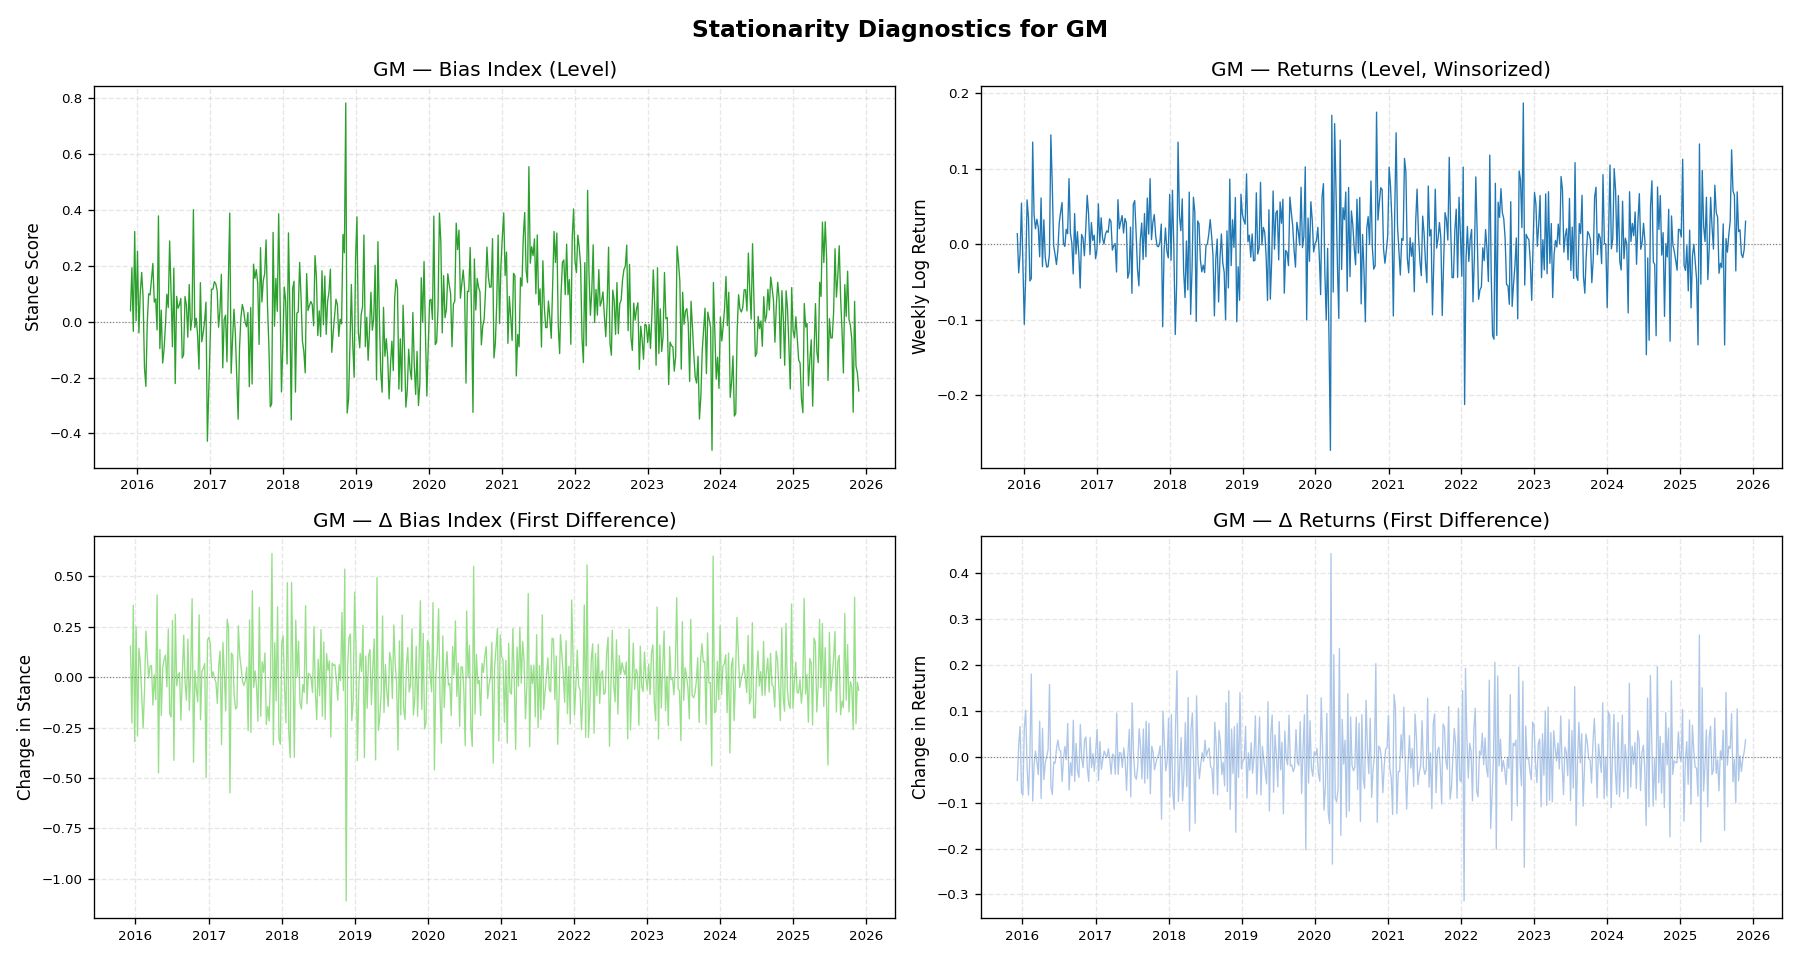
\includegraphics[width=\columnwidth]{fig_stationarity_GM.png}}
\caption{Stationarity diagnostics for General Motors (GM): the bias index and
weekly return in levels (left) and first differences (right), with ADF and KPSS
verdicts driving the integration-order classification.}
\label{fig:stat}
\end{figure}

\subsection{Stage 6: Structural Break Testing}
Because the central hypothesis concerns a regime change around 2020, we date
breaks empirically rather than imposing the calendar. A Bai--Perron procedure,
implemented by dynamic programming for a single change point under an $L_2$
(mean-shift) cost, locates the largest structural shift in the mean of each
weekly series. The estimated bias-index break dates serve as the
\texttt{is\_post\_break} cut used to split the sample for the subsequent
subsample Granger tests, and every firm yields a valid split with at least $60$
observations on each side. Figures~\ref{fig:breakV} and~\ref{fig:breakWFC} show
the data-driven breaks for two firms; several cluster near the COVID window while
others reflect firm-specific events, which is itself evidence that a single
imposed 2020 dummy would be too blunt.

\begin{figure}[!t]
\centerline{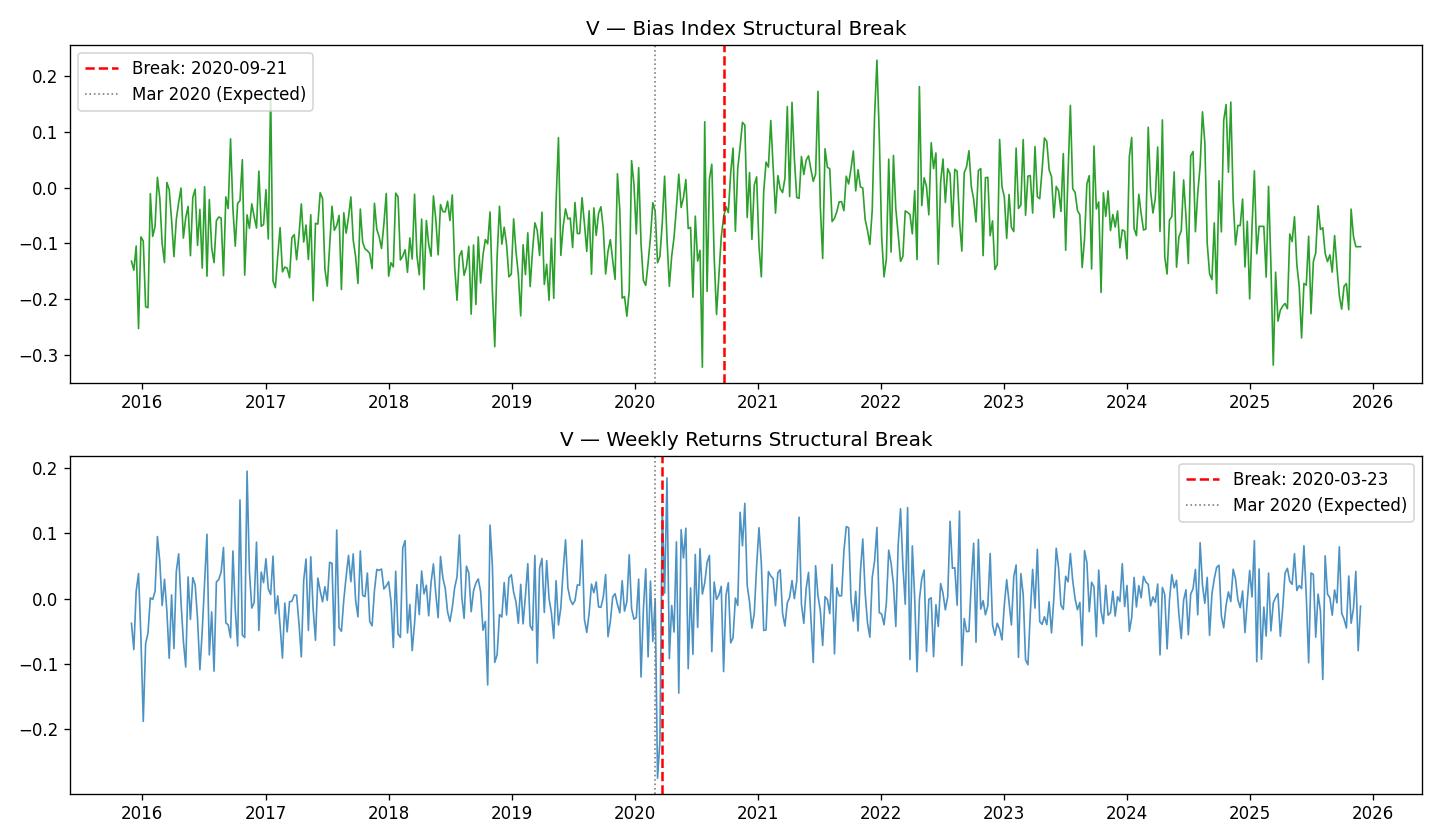
\includegraphics[width=\columnwidth]{fig_breaks_V.png}}
\caption{Bai--Perron structural breaks for Visa (V). The return break
(2020-03-23) coincides with the COVID crash; the bias break (2020-09-21) lags it.}
\label{fig:breakV}
\end{figure}

\begin{figure}[!t]
\centerline{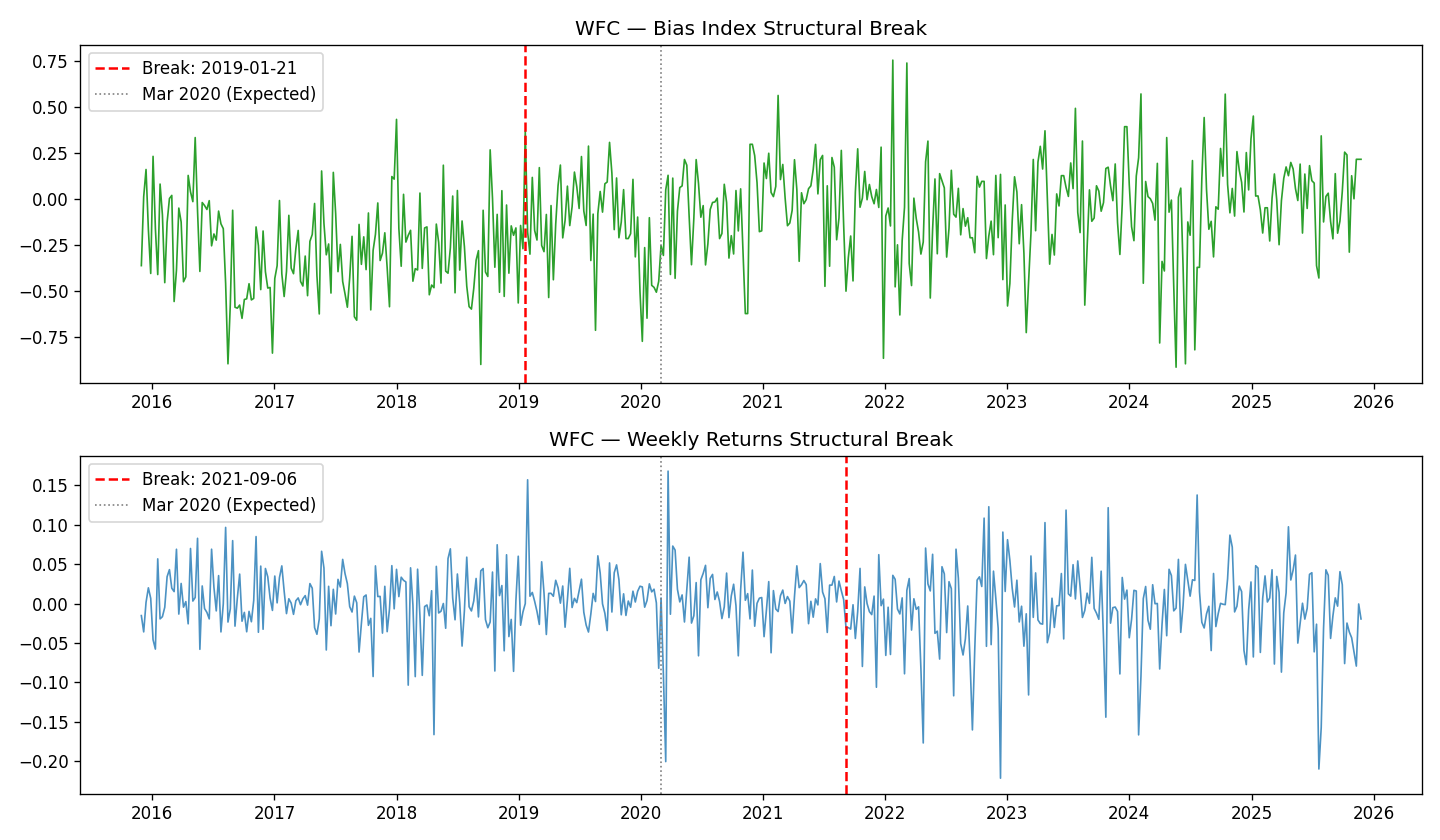
\includegraphics[width=\columnwidth]{fig_breaks_WFC.png}}
\caption{Bai--Perron structural breaks for Wells Fargo (WFC), the one firm with a
cointegrating bias--return relation and significant full-sample causality.}
\label{fig:breakWFC}
\end{figure}

\subsection{Stage 7: VAR Specification}
For each firm the VAR order is selected by estimating
Eq.~\eqref{eq:var} for $p=1,\dots,8$ and minimizing the Bayesian Information
Criterion (BIC), which penalizes parameters more heavily than AIC and so favors
parsimonious, well-identified models; when BIC selects zero lags we impose $p=1$
to retain a dynamic model. The selected orders range from $1$ to $5$ (modal
value $p=3$). Three residual diagnostics certify each fit. Stability requires
all roots of the companion matrix to lie outside the unit circle, equivalent to
$\det(\mathbf{I}-\sum_\ell \mathbf{A}_\ell z^\ell)\ne 0$ for $|z|\le 1$; every
selected model is stable (minimum root $>1.28$). The Portmanteau test checks for
residual autocorrelation, confirming the chosen lag is adequate for most firms.
The Jarque--Bera test rejects normality everywhere, the familiar heavy-tail
signature of financial data, which leaves VAR coefficients consistent but
motivates robust inference; Engle's ARCH test detects volatility clustering in
several return residuals, reinforcing the use of HAC-robust standard errors in
the causality stage.

\subsection{Stage 8: Granger Causality}
Granger causality operationalizes ``does past $X$ help predict $Y$ beyond $Y$'s
own past.'' Stance Granger-causes returns if the lagged stance coefficients are
jointly nonzero in the return equation, i.e. $H_0:\,a^{(2,1)}_1=\dots=a^{(2,1)}_p=0$
is rejected. We test this with a direct OLS regression of each variable on $p$
lags of both variables, using a joint Wald ($F$) test and Newey--West HAC-robust
standard errors (\texttt{maxlags}$=p$) to neutralize the heteroscedasticity and
autocorrelation found in Stage 7. Table~\ref{tab:granger} reports the
firm-level full-sample $p$-values. Causality is sparse in the full sample, as
expected if the relationship is regime-dependent: stance Granger-causes returns
for Wells Fargo ($p=0.023$) and weakly for Morgan Stanley ($p=0.058$), and the
reverse direction (returns to bias) is significant for Goldman Sachs
($p=0.012$).

\begin{table}[!t]
\caption{Firm-Level Granger Causality, Full Sample (HAC $p$-values)}
\label{tab:granger}
\centering
\small
\begin{tabular}{lrrr}
\toprule
Firm & Lag & Bias$\to$Ret & Ret$\to$Bias \\
\midrule
GS  & 5 & $0.757$ & $0.012$ \\
MS  & 3 & $0.058$ & $0.193$ \\
WFC & 5 & $0.023$ & $0.307$ \\
\multicolumn{4}{l}{\textit{Other 12 firms: no direction significant at $5\%$.}}\\
\bottomrule
\end{tabular}
\end{table}

The more informative test splits each firm at its empirical bias break and
re-estimates causality on each side. Several firms that are quiet in the full
sample show post-break causality that is absent pre-break: Wells Fargo
(bias$\to$returns $p=0.013$ post versus $0.345$ pre) and Morgan Stanley
(bias$\to$returns $p=0.052$ post) are the clearest cases, with feedback
(returns$\to$bias) emerging post-break for Boeing, Goldman Sachs, and Morgan
Stanley. This pre/post asymmetry is the firm-level analogue of the structural
shift the regressions probe: the media--market link is not constant but switches
on after the break for a subset of firms.

\subsection{Panel VAR}
Firm-by-firm tests are underpowered because each uses only one short series. We
therefore pool the cross-section into a panel VAR, which is the design the study
most relies on for its dynamic conclusion. Unobserved firm heterogeneity is
removed with the Arellano--Bover/Helmert transformation (forward
mean-differencing), which subtracts from each observation the mean of all its
\emph{future} values within the firm,
\begin{equation}
\tilde{y}_{it} = c_{it}\Bigl(y_{it} - \tfrac{1}{T_{it}}\textstyle\sum_{s>t} y_{is}\Bigr),
\end{equation}
with a scaling factor $c_{it}$ that equalizes the variance of the transformed
errors. Unlike ordinary within-demeaning, this transformation preserves the
orthogonality between the transformed variables and the lagged regressors,
avoiding the look-ahead bias (Nickell bias) that contaminates dynamic
fixed-effects panels. The endogenous variables are again $\Delta\text{bias}$ and
the weekly log return; we additionally partial out the exogenous controls
$\text{Post}_t$, VIX, the S\&P 500 weekly log return, and the article count
$N_{\text{articles}}$, so that any detected causality cannot be attributed to
market-wide volatility or coverage volume. With $p=3$ lags and HAC-robust
standard errors, the pooled model is estimated by OLS on the transformed,
constant-free data, and Granger directions are tested with joint Wald statistics
over the full, pre-break, and post-break samples. Table~\ref{tab:panelvar}
reports the results.

\begin{table}[!t]
\caption{Panel VAR Granger Causality (15 firms, Helmert-transformed, HAC)}
\label{tab:panelvar}
\centering
\small
\begin{tabular}{lrrr}
\toprule
Sample & $N$ & Bias$\to$Ret & Ret$\to$Bias \\
\midrule
Full        & $7493$ & $0.976$ & $0.200$ \\
Pre-break   & $4168$ & $0.245$ & $0.801$ \\
Post-break  & $3265$ & $0.617$ & $0.187$ \\
\bottomrule
\end{tabular}
\end{table}

Pooling buys power but, even so, neither Granger direction is significant at
conventional levels in any subsample once VIX, the index return, and article
volume are controlled. The honest reading is that the firm-level post-break
signals for Wells Fargo and Morgan Stanley do not aggregate into a uniform
panel-wide media-to-returns channel: the dynamic link, where it exists, is
firm-specific and heterogeneous rather than a market-wide regularity. This
strengthens rather than weakens the contribution, because the panel VAR is
exactly the test that would manufacture a spurious aggregate effect if the
controls were omitted, and it declines to do so.

\subsection{Limitations of the VAR Pipeline}
Several caveats bound the dynamic findings. A weekly frequency, chosen for
coverage, may be too coarse to capture the intraday or daily horizon over which
news is plausibly priced, so a true fast media-to-price channel could be
aliased away by aggregation. The single-break Bai--Perron design dates exactly
one change point per series; firms with multiple regime shifts are only partially
described, and the break date is estimated with sampling error that the
subsample split treats as known. The bivariate VAR omits other drivers of both
stance and returns (earnings surprises, analyst actions, sector shocks), so the
controls in the panel model mitigate but do not eliminate omitted-variable
concerns. Heavy-tailed, volatility-clustered residuals mean small-sample
inference leans on the HAC correction and asymptotics rather than exact
distributions. Finally, Granger causality is predictive, not structural: a
significant test says past stance forecasts returns, not that stance
mechanically moves prices, and the firm-specific nature of the surviving signals
counsels caution against a universal causal claim.

\section{Identification, Validity, and Robustness}
We address three main threats. First, macro shocks may move both coverage and prices; we control with index returns and VIX. Second, article volume differs widely across firms; we include volume covariates and run trimmed samples. Third, parallel trends may not hold; we use pre-trend checks, placebo cutoffs, and SCDiD when needed.

Robustness checks include alternate stance thresholds (0.9, 0.6, 0.0), alternative aggregation (mean vs median), lagged stance controls, sector controls, and quantile regressions to test for tail effects in returns.

\section{Conclusion and Next Steps}
This draft provides a full narrative of the project to date: why the 2020 shock matters, how we build a target-dependent stance signal, and how we test for structural changes and market effects. Next steps include finalizing the firm panel, completing the relevance classifier evaluation, computing the daily stance series, and running the full RQ1--RQ3 specifications with robustness tables and figures.

\bibliographystyle{IEEEtran}
\begin{thebibliography}{99}
\bibitem{hamborg2021} F. Hamborg and K. Donnay, ``NewsMTSC: Target-dependent stance classification in news articles,'' EACL, 2021.
\bibitem{haroon2020} O. Haroon and S. A. Rizvi, ``COVID-19: Media coverage and financial markets behavior,'' Finance Research Letters, 2020.
\bibitem{blajer2024} M. Blajer-Golebiewska, A. Honecker, and K. Nowak, ``Investor sentiment response to COVID-19: A sectoral analysis,'' North American Journal of Economics and Finance, 2024.
\bibitem{news2024} ``News and markets in the time of COVID-19,'' Journal of Financial and Quantitative Analysis, 2024.
\bibitem{davis2020} S. Davis, S. Hansen, and C. Seminario, ``Firm-level risk exposures and stock returns in the wake of COVID-19,'' NBER, 2020.
\bibitem{costola2023} M. Costola, M. Nofer, O. Hinz, and L. Pelizzon, ``Machine learning sentiment analysis, COVID-19 news and stock market reactions,'' Research in International Business and Finance, 2023.
\bibitem{bai2023} Z. Bai, Q. Han, J. Pan, and R. Zhang, ``Financial market sentiment and returns,'' Finance Research Letters, 2023.
\bibitem{xu2024} H. Xu, ``News bias in financial journalists' social networks,'' Journal of Accounting Research, 2024.
\end{thebibliography}

\end{document}